\documentclass[10pt,a4paper]{article}
\usepackage[margin=19mm,top=21mm,bottom=20mm]{geometry}
\usepackage[T1]{fontenc}
\usepackage[utf8]{inputenc}
\usepackage{lmodern,microtype}
\DeclareUnicodeCharacter{2212}{\ensuremath{-}}
\usepackage{babel}
\babelprovide[main,import]{romanian}
\usepackage{multicol,booktabs,graphicx,amsmath,xcolor,caption,fancyhdr,titlesec,ragged2e}
\usepackage{hyperref}
\definecolor{accent}{HTML}{24576B}
\hypersetup{colorlinks=true,linkcolor=accent,urlcolor=accent,citecolor=accent,
pdftitle={Clasificarea expresiilor faciale cu HOG, SVM și învățare prin transfer},
pdfauthor={Colăcel Cristian-Adrian}}
\pdfinfoomitdate=1
\renewcommand{\thesection}{\Roman{section}}
\titleformat{\section}{\large\bfseries\color{accent}}{\thesection.}{.5em}{}
\titleformat{\subsection}{\normalsize\bfseries}{}{0pt}{}
\titlespacing*{\section}{0pt}{9pt}{8pt}
\titlespacing*{\subsection}{0pt}{8pt}{4pt}
\setlength{\columnsep}{8mm}
\setlength{\parindent}{0pt}
\setlength{\parskip}{5pt}
\setlength{\emergencystretch}{2em}
\captionsetup{font=small,labelfont=bf,skip=5pt,hypcap=false,justification=raggedright,singlelinecheck=false}
\pagestyle{fancy}\fancyhf{}
\fancyhead[L]{\small Clasificarea expresiilor faciale}
\fancyhead[R]{\small HOG / ResNet18 / SVM}
\fancyfoot[C]{\thepage}
\renewcommand{\headrulewidth}{0.2pt}
\setlength{\headheight}{14pt}
\begin{document}
\thispagestyle{plain}
\begin{center}
{\LARGE\bfseries Clasificarea expresiilor faciale\par}
\vspace{5pt}
{\Large cu HOG, SVM și învățare prin transfer\par}
\vspace{8pt}
Studiu educațional de evaluare reproductibilă\\[5pt]
Colăcel Cristian-Adrian
\end{center}
\vspace{5pt}
\textbf{Rezumat.} Studiul compară descriptori HOG și trăsături extrase de un
ResNet18 preantrenat, folosind aceleași clasificatoare SVM și aceeași procedură
de evaluare. Conținutul celor 3000 de imagini este identificat în FER2013 prin
amprente digitale, iar grupurile cunoscute de duplicate sunt tratate înaintea împărțirii.
Experimentul folosește 2069 de imagini pentru dezvoltare și 509 pentru evaluare
separată. Cele două variante RBF obțin aceeași acuratețe, 39,49\%, dar au
comportamente diferite pe clase. Predicțiile individuale și verificările
salvate permit recalcularea rezultatelor.
\begin{multicols}{2}\RaggedRight
\section{Scop și contribuție}
Proiectul urmărește cum se schimbă clasificarea atunci când aceeași imagine
este descrisă prin contururi locale sau printr-o reprezentare învățată anterior.
Ambele reprezentări folosesc SVM liniar și SVM cu nucleu RBF, cu același buget
de selecție a parametrilor. SVM liniar folosește frontiere liniare în
spațiul caracteristicilor, iar nucleul RBF permite frontiere neliniare.

Contribuția proprie este organizarea experimentului: identificarea sursei,
manifestul pe imagini, evidența excluderilor, împărțirile comune și legătura
între predicții și raport. HOG, SVM și ResNet sunt metode consacrate.

Ținta este eticheta expresiei din setul de date: furie, dezgust, frică, bucurie,
neutru, tristețe sau surpriză. Aceste denumiri nu sunt măsurători ale stării
emoționale interioare a persoanei~\cite{barrett}.

\subsection{Două reprezentări}
\textbf{HOG} descrie orientarea contururilor din regiuni mici ale
imaginii~\cite{hog}. Configurația folosește nouă orientări, celule de
8$\times$8 pixeli, blocuri de 2$\times$2 celule și normalizare L2-Hys.
Intensitățile sunt împărțite la 255; vectorul rezultat are 900 de valori.

\textbf{ResNet18} extrage 512 caracteristici cu ponderile oficiale
ImageNet1K V1~\cite{resnet}. Rețeaua este fixată în modul de evaluare, fără
reantrenarea ponderilor pe imaginile faciale. Transformările convertesc la
RGB, redimensionează latura scurtă la 256, decupează central 224$\times$224
și aplică normalizarea ImageNet.

Reprezentările diferă prin dimensiune, cost și accesul la informația din
preantrenare. Experimentul controlează clasificatorul și datele, fără a
egaliza aceste avantaje.

\columnbreak
\section{Date și proveniență}
Arhiva academică include 3000 de imagini JPEG alb-negru, de 48$\times$48
pixeli. Sunt disponibile 2700 de etichete. Celelalte 300 de imagini formează
setul academic pentru predicție și nu intră în calculul scorurilor.

Fiecare fișier are un corespondent identic în distribuția Kaggle
\texttt{msambare/fer2013}, versiunea 1~\cite{kaggle}. Potrivirea folosește
amprenta digitală SHA-256 a întregului fișier: aceeași valoare identifică
fișiere identice, nu doar imagini asemănătoare. Contextul FER2013 este
descris în raportul competiției originale~\cite{fer}.

Distribuția indică ODbL pentru baza de date și DbCL pentru conținut.
Declarația nu certifică independent drepturile fiecărei fotografii~\cite{license}.
Documentul prezintă rezultate agregate, fără fotografii.

\subsection{Tratarea duplicatelor}
Auditul exact identifică 20 de grupuri cu 42 de imagini. Șapte grupuri
traversează împărțirea istorică de antrenare și validare. O fotografie
reutilizată în ambele seturi poate favoriza memorarea, de aceea gruparea
precedă evaluarea~\cite{duplicates}.

O căutare de imagini similare produce 126 de perechi candidate. Revizuirea
vizuală clasifică 37 drept aproape duplicate, 87 drept imagini diferite și
două drept incerte. Sunt excluse 23 de imagini etichetate: 13 din grupuri
cu etichete contradictorii, trei din grupuri incerte și încă șapte legate
de setul academic fără etichete. Rămân 2677 de imagini eligibile.

Copiile cunoscute cu aceeași etichetă rămân împreună. Revizuirea unică
poate omite copii transformate. Fără identificatori de persoane, gruparea
controlează reutilizarea imaginilor, nu separarea tuturor fotografiilor
aceleiași persoane.
\end{multicols}

\newpage
\section{Protocolul de evaluare}
Subsetul academic amestecă partițiile distribuției FER2013. Dintre cele 3000
de imagini, 2324 apar exclusiv în partiția sursei pentru antrenare, 562
exclusiv în cea pentru test și 114 în ambele, prin copii exacte. Selecția
folosește apartenența verificată a conținutului.
\begin{center}
\begin{tabular}{lr}\toprule
Selecție din inventarul de 2677 de imagini eligibile & Imagini \\\midrule
Dezvoltare: exclusiv în partiția de antrenare a sursei & 2069 \\
Excluse: conținut exact în ambele partiții ale sursei & 96 \\
Excluse: grup cunoscut prezent și în dezvoltare & 3 \\
Evaluare separată: exclusiv în partiția de test a sursei & 509 \\\bottomrule
\end{tabular}
\captionof{table}{Separarea după sursă și grupurile cunoscute de imagini.}
\end{center}
\begin{multicols}{2}\RaggedRight
\subsection{Selecția parametrilor}
Cele 2069 de imagini de dezvoltare sunt împărțite în cinci subseturi. La fiecare pas se antrenează pe patru și se prezice al
cincilea. Fiecare imagine primește o singură predicție de la un model care
nu a folosit-o la antrenare. Rezultatele reunite sunt denumite
\emph{validare încrucișată} în tabele și grafice.

În interiorul fiecărui set de antrenare, alte trei subseturi selectează
parametrul $C$ dintre 0,1; 1 și 10. Se maximizează media macro-F1 internă,
preferând $C$ mai mic la egalitate. Grupurile cunoscute rămân împreună la
ambele niveluri ale împărțirii.

Pentru cele 509 imagini separate se selectează $C$ prin trei subseturi numai
în dezvoltare, apoi se ajustează modelul pe toate cele 2069 de imagini.
Setul separat nu participă la această antrenare sau selecție.

\subsection{Standardizare și reper simplu}
StandardScaler estimează media și dispersia fiecărei caracteristici numai
pe antrenarea subsetului de antrenare curent. Transformarea se aplică apoi imaginilor
evaluate, evitând folosirea distribuției lor la ajustarea scalerului.

SVM liniar și SVM RBF folosesc aceleași valori candidate pentru $C$;
varianta RBF are \texttt{gamma=scale}. Ca reper, predictorul majoritar
atribuie tuturor imaginilor clasa cea mai frecventă din antrenare: bucurie.
El arată cât se poate obține fără analiza pixelilor.

\subsection{Ce descrie experimentul}
Evaluarea separată este retrospectivă: imaginile etichetate au fost
accesibile în etape anterioare ale proiectului. Protocolul controlează
antrenarea curentă, dar nu reprezintă un test istoric neatins sau rezultatul
pe întregul set de referință FER2013. Scorurile istorice pe alte împărțiri rămân
documentate separat.

\columnbreak
\subsection{Metrici și interpretare}
\textbf{Acuratețea} este proporția tuturor predicțiilor corecte.
\textbf{Rata de recunoaștere} (recall) arată ce proporție dintre imaginile
unei clase este recunoscută corect. \textbf{Precizia} arată câte dintre predicțiile
atribuite clasei sunt corecte.

Scorul F1 combină precizia $P$ și rata de recunoaștere $R$:
\[
 F1=\frac{2PR}{P+R},\qquad
 \text{macro-F1}=\frac{1}{7}\sum_{c=1}^{7}F1_c.
\]
Se folosește zero când numitorul este nul. Macro-F1 acordă pondere egală
celor șapte clase și este criteriul principal al selecției. O clasă rară
nu dispare astfel în spatele scorului bun pe clasa majoritară.

Matricea de confuzie detaliază predicțiile fiecărei clase: rândurile sunt
etichetele de referință, coloanele sunt predicțiile, iar diagonala conține
clasificările corecte. Numărul imaginilor din clasă este afișat în tabelul pe clase.

\subsection{Incertitudinea diferențelor}
Intervalele folosesc 2000 de resamplări bootstrap. Se aleg cu înlocuire
grupuri cunoscute în interiorul fiecărei clase; aceeași selecție este
aplicată tuturor modelelor. Se calculează astfel intervale pentru scoruri
și pentru diferența dintre două modele.

Intervalele descriu variația predicțiilor salvate la resamplarea imaginilor.
Nu reantrenează modelele și nu includ variația altor împărțiri sau selecții
de parametri. În validarea încrucișată există și dependență între modele,
deoarece antrenările lor se suprapun; bootstrap-ul folosit nu o include~\cite{cv}.

\subsection{Verificarea rezultatelor}
Manifestul leagă fiecare ID de etichetă, fișier și grup. Metricile sunt
recalculate din predicțiile salvate, iar predicțiile finale sunt reproduse
din modelele păstrate. Verificările controlează separarea grupurilor și
folosirea exclusivă a imaginilor de antrenare la ajustarea scalerelor.
\end{multicols}

\newpage
\section{Rezultate comparative}
\begin{center}
\begin{tabular}{lrrrr}
\toprule
& \multicolumn{2}{c}{Validare încrucișată} & \multicolumn{2}{c}{Evaluare separată} \\
\cmidrule(lr){2-3}\cmidrule(lr){4-5}
Model & Acuratețe (\%) & Macro-F1 & Acuratețe (\%) & Macro-F1 \\
\midrule
Majoritar & 24,55 & 0,0563 & 24,75 & 0,0567 \\
HOG + SVM liniar & 28,66 & 0,2520 & 30,84 & 0,2758 \\
HOG + SVM RBF & 39,29 & 0,3096 & 39,49 & 0,3157 \\
ResNet18 + SVM liniar & 37,60 & 0,3263 & 33,99 & 0,3011 \\
ResNet18 + SVM RBF & 44,03 & 0,3692 & 39,49 & 0,3528 \\
\bottomrule
\end{tabular}

\captionof{table}{Predicții pe aceleași imagini pentru toate modelele:
2069 în validarea încrucișată și 509 în evaluarea separată.}
\end{center}
\vspace{5pt}
\begin{center}
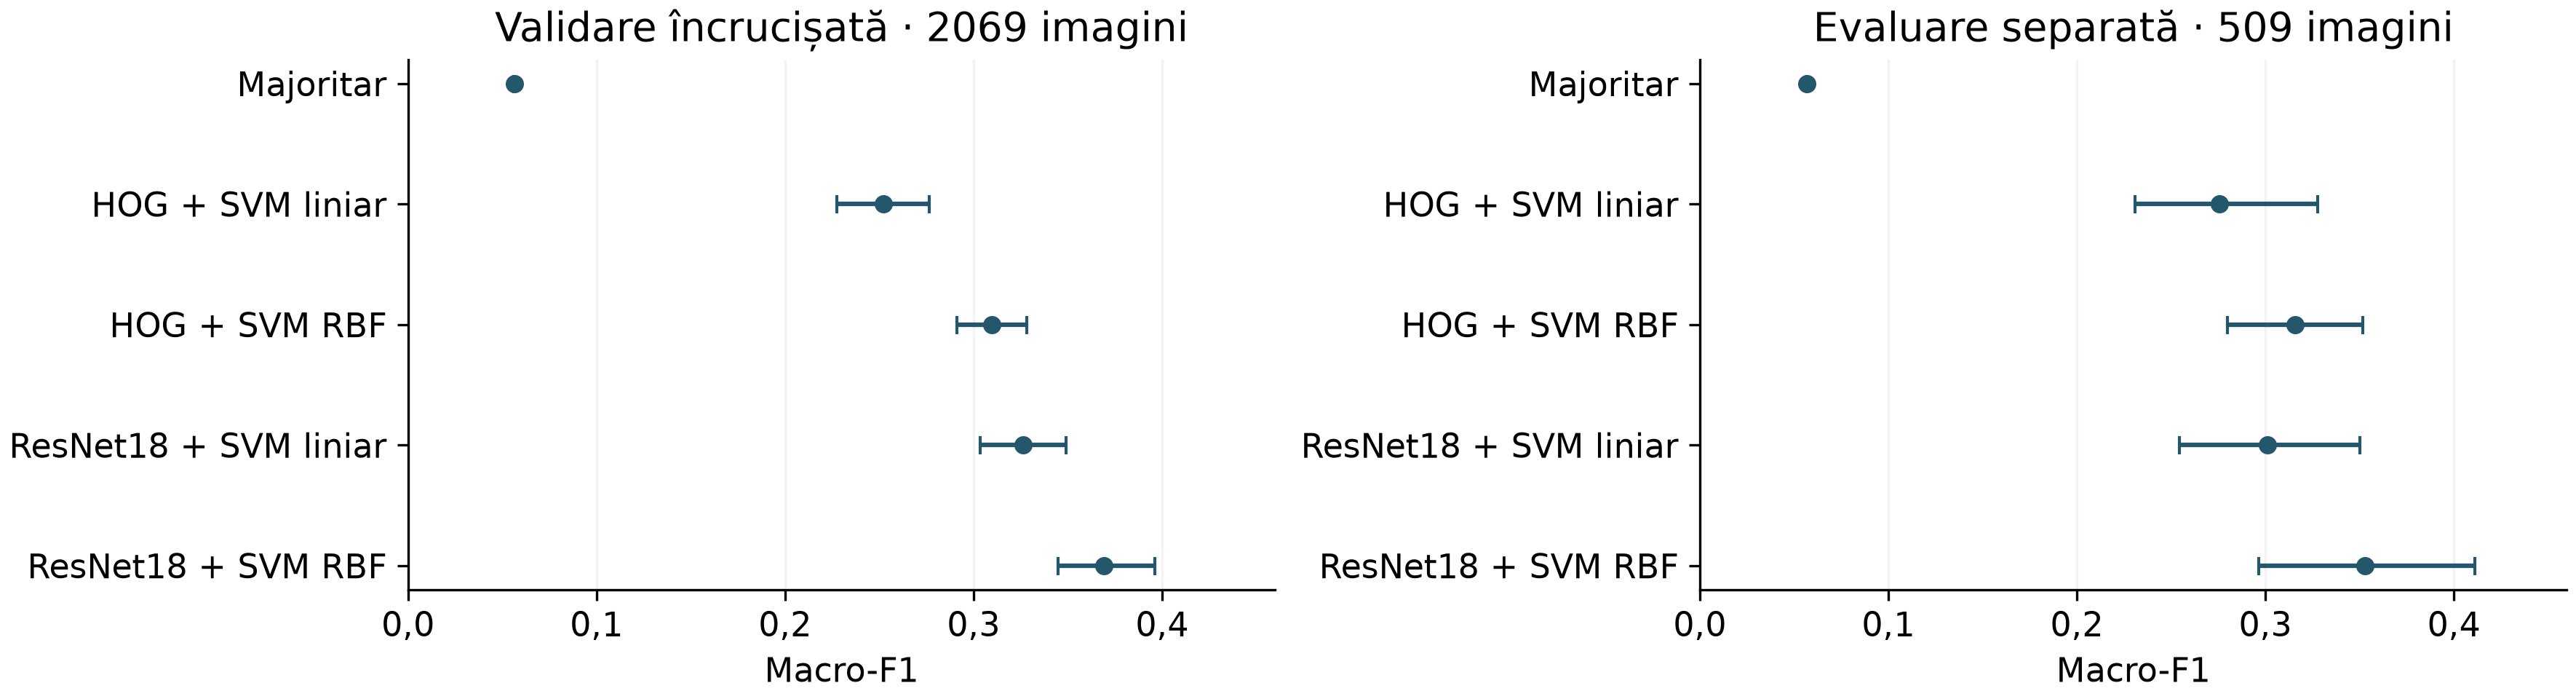
\includegraphics[width=\linewidth]{figuri/macro_f1_ro.png}
\captionof{figure}{Macro-F1 și intervale bootstrap de 95\%, condiționate de
predicțiile salvate. Punctul este scorul, iar segmentul este intervalul.}
\end{center}
\begin{multicols}{2}\RaggedRight
\subsection{Reprezentarea și clasificatorul}
În validarea încrucișată, ResNet18 cu SVM RBF obține cel mai mare macro-F1
dintre configurațiile testate: 0,3692. HOG cu același tip de SVM obține
0,3096. Diferența este 0,0596, cu interval pereche de 95\%
[0,0317; 0,0876], în sensul condiționat explicat în protocol.

Alegerea clasificatorului contează pentru ambele reprezentări. Înlocuirea
SVM liniar cu RBF crește macro-F1 de la 0,2520 la 0,3096 pentru HOG și
de la 0,3263 la 0,3692 pentru ResNet18. Reprezentarea este astfel evaluată
împreună cu tipul de SVM folosit.

Parametrii selectați pe întreaga dezvoltare sunt $C=0,1$ pentru ambele
variante liniare și $C=10$ pentru ambele RBF.

\subsection{Ce arată reperul majoritar}
Predictorul majoritar are 24,75\% acuratețe pe setul separat, dar numai
0,0567 macro-F1. El recunoaște exclusiv bucuria, cea mai frecventă clasă.
Diferența dintre metrici arată de ce acuratețea singură este insuficientă
pentru acest eșantion dezechilibrat.

\columnbreak
\subsection{Aceeași acuratețe, erori diferite}
Pe cele 509 imagini separate, HOG-RBF și ResNet18-RBF clasifică fiecare
corect 201 imagini: 39,49\% acuratețe. Macro-F1 este însă 0,3157 pentru
HOG și 0,3528 pentru ResNet18, deoarece erorile sunt distribuite diferit
între clase.

Diferența macro-F1 ResNet18 minus HOG este 0,0371. Intervalul pereche de
95\% este [−0,0235; 0,0972] și include zero. În acest eșantion, diferența
observată nu susține o concluzie fermă de superioritate între variantele RBF.

\subsection{Costul calculului}
Rularea completă a durat 114,80 secunde, incluzând extragerea
caracteristicilor, 240 de ajustări SVM, predicțiile și bootstrap-ul.
Extragerea pe toate cele 2578 de imagini active a durat 0,95 secunde
pentru HOG și 27,18 secunde pentru ResNet18.

Trăsăturile fixe sunt calculate o singură dată și reutilizate; scalerele
sunt ajustate separat în fiecare antrenare. Măsurarea folosește un
Intel Core i5-13600KF, fără CUDA și cu maximum patru fire Torch. Timpii
descriu o rulare pe loturi, nu latența unei aplicații interactive.
\end{multicols}

\newpage
\section{Analiza erorilor pe clase}
\begin{center}
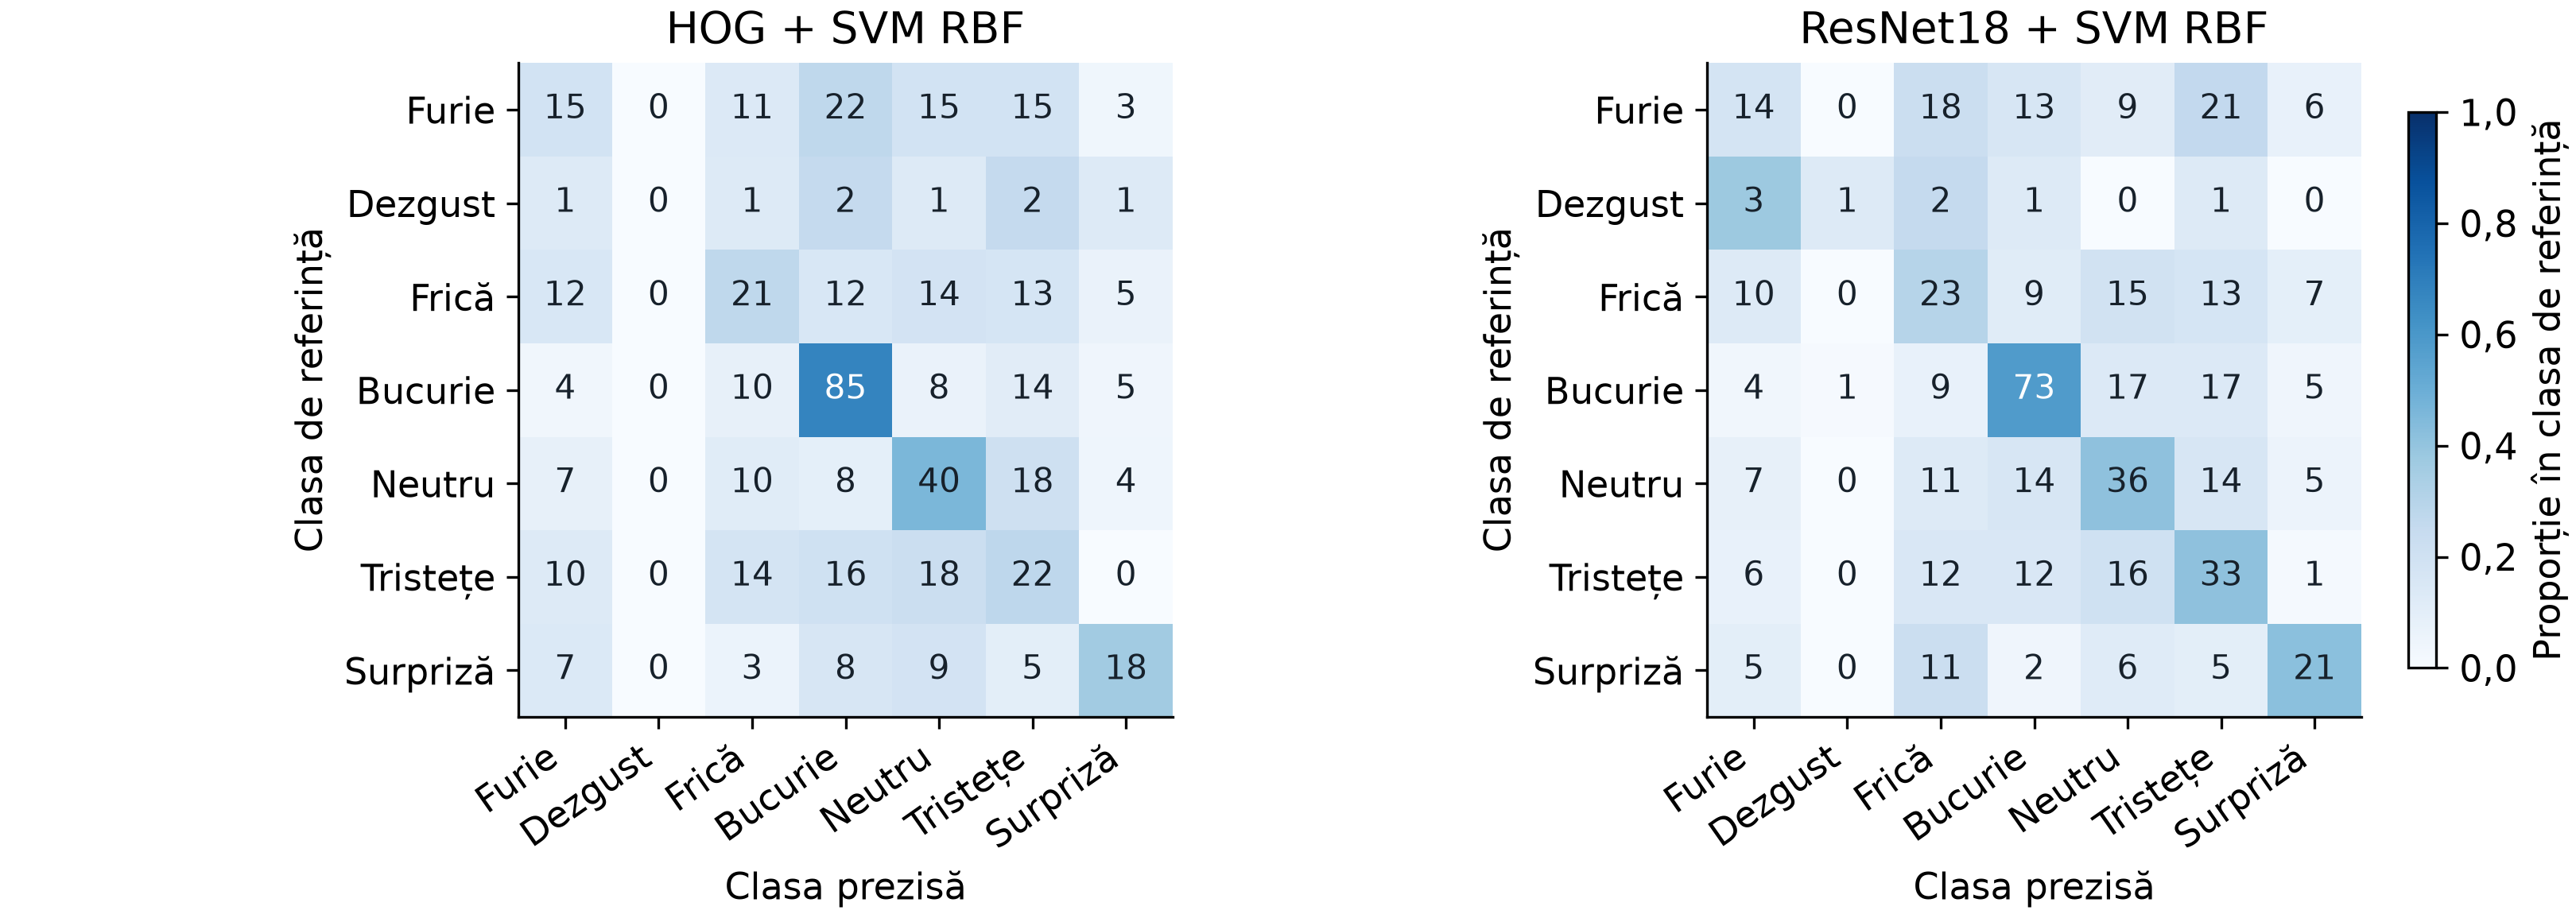
\includegraphics[width=\linewidth]{figuri/confuzii_rbf_ro.png}
\captionof{figure}{Cele două modele RBF pe setul separat. Numerele sunt
imagini; culoarea arată proporția în fiecare clasă de referință. Matricele
celorlalte două modele se află în exporturile numerice.}
\end{center}
\begin{center}
\begin{tabular}{lrrrrr}
\toprule
Clasă & Imagini & HOG liniar & HOG RBF & ResNet liniar & ResNet RBF \\
\midrule
Furie & 81 & 22,2 & 18,5 & 28,4 & 17,3 \\
Dezgust & 8 & 12,5 & 0,0 & 12,5 & 12,5 \\
Frică & 77 & 33,8 & 27,3 & 33,8 & 29,9 \\
Bucurie & 126 & 42,9 & 67,5 & 47,6 & 57,9 \\
Neutru & 87 & 32,2 & 46,0 & 35,6 & 41,4 \\
Tristețe & 80 & 21,2 & 27,5 & 21,2 & 41,2 \\
Surpriză & 50 & 26,0 & 36,0 & 30,0 & 42,0 \\
\bottomrule
\end{tabular}

\captionof{table}{Rata de recunoaștere în procente și numărul de imagini din fiecare clasă.}
\end{center}
\begin{multicols}{2}\RaggedRight
\subsection{Citirea confuziilor}
ResNet18-RBF recunoaște 33 dintre cele 80 de imagini de tristețe, față
de 22 pentru HOG-RBF. Pe bucurie, ordinea se inversează: 73 dintre 126,
față de 85. Câștigul nu este uniform pe clase.

Dezgustul are numai opt imagini. HOG-RBF nu recunoaște niciuna, iar
ResNet18-RBF recunoaște una. Fiecare imagine schimbă rata cu 12,5
puncte procentuale; procentul trebuie citit împreună cu acest suport mic.

\subsection{Concluzie și reproducere}
Studiul urmărește comparația de la imaginea verificată până la predicție
și metrică. Controlul clasificatorului schimbă interpretarea comparației
HOG--ResNet18, iar analiza pe clase explică de ce aceeași acuratețe poate
ascunde scoruri macro-F1 diferite.

Manifestele, predicțiile și instrucțiunile sunt disponibile în
\href{https://github.com/colacbrr/Real-Time-Emotion-Recognition-Platform}{repository-ul proiectului}.
Comanda \texttt{python scripts/verify\_published\_results.py}
verifică integritatea exporturilor și recalculează metricile fără imagini
sau ponderi. Refacerea antrenării necesită imaginile și ponderile
verificate. Figurile și tabelele provin din rezultatele salvate.

\columnbreak
\small
\renewcommand{\refname}{Referințe}
\begin{thebibliography}{8}
\setlength{\itemsep}{4pt}\setlength{\parskip}{0pt}
\bibitem{fer} I. J. Goodfellow et al. \emph{Challenges in Representation
Learning: A report on three machine learning contests.}
\href{https://arxiv.org/abs/1307.0414}{arXiv:1307.0414}.
\bibitem{hog} N. Dalal, B. Triggs. \emph{Histograms of Oriented Gradients
for Human Detection.} CVPR, 2005, pp. 886--893.
\bibitem{resnet} K. He et al. \emph{Deep Residual Learning for Image
Recognition.} CVPR, 2016, pp. 770--778.
\href{https://arxiv.org/abs/1512.03385}{Text integral}.
\bibitem{kaggle} M. Sambare. \emph{FER-2013}, distribuția Kaggle, versiunea 1.
\href{https://www.kaggle.com/datasets/msambare/fer2013}{Dataset și metadate}.
\bibitem{duplicates} B. Barz, J. Denzler. \emph{Do We Train on Test Data?
Purging CIFAR of Near-Duplicates.} Journal of Imaging 6(6):41.
\href{https://doi.org/10.3390/jimaging6060041}{Text integral}.
\bibitem{cv} Y. Bengio, Y. Grandvalet. \emph{No Unbiased Estimator of the
Variance of K-Fold Cross-Validation.} JMLR 5:1089--1105.
\href{https://jmlr.org/papers/v5/grandvalet04a.html}{Text integral}.
\bibitem{barrett} L. F. Barrett et al. \emph{Emotional Expressions
Reconsidered: Challenges to Inferring Emotion From Human Facial Movements.}
\href{https://doi.org/10.1177/1529100619832930}{Articol}.
\bibitem{license} Open Data Commons:
\href{https://opendatacommons.org/licenses/odbl/1-0/}{ODbL 1.0} și
\href{https://opendatacommons.org/licenses/dbcl/1-0/}{DbCL 1.0}.
\end{thebibliography}
\end{multicols}
\end{document}
